\section{Introducción}
En el anterior artículo de esta serie vimos cómo representar una función periódica como suma de armónicos, idea que desarrolló Fourier cuando quiso explicar cómo se propagaba el calor. Sin embargo, esa técnica resultó ser fácilmente extrapolable a problemas de otras ramas de la física e ingenería, como la teoría de circuitos eléctricos.

A lo largo de este artículo iremos aplicando la estrategia que desarrolló Fourier a un clásico problema de electromagnetismo, el circuito RLC (resistor-inductor-capacitor circuit). De hecho, tras una primera aproximación utilizando senos y cosenos, volveremos a mirar el problema bajo el prisma del análisis complejo, viendo como el problema se simplifica aún más.

Si queréis ampliar, os recomendamos que consultéis \cite{Sadiku}, pues es el libro que seguiremos en este artículo.

\section{El circuito RLC}
Vamos a comenzar planteando detalladamente el problema que queremos resolver. Tenemos el circuito mostrado en la Figura \ref{fig:RLC}, formado por una resistencia que denotamos por $R$, una bobina con inducción $L$ y un condensador con capacidad $C$, con todos los elementos dispuestos en serie.
\begin{figure}[h]
\begin{figurebox}
    \vspace{5pt}
    \centering
         \scalebox{1}{%
%
% Con esto ajusto el tamaño de los componentes
\ctikzset{ bipoles/length=1.3cm}
\begin{circuitikz}[scale=1]%\shorthandoff{>}
% Rama izquierda
    \def\xa{0}
    \def\ya{0}
    \def\xb{1.5}
    \def\yb{3}
    \draw                                     (\xa,\ya)
             to[american voltage source]      (\xa,\yb)
             to[short, -*]                    (\xb,\yb)
             to[open]                         (\xb,\ya)
             to[short, *-]                    (\xa,\ya);
%
%
% Bloque central
    \def\xc{8}
    \def\yc{3.5}
    \def\yd{-0.3}
    \draw [dotted]                            (\xb,\yc)
             to[dotted]                       (\xc,\yc)
             to[dotted]                       (\xc,\yd) 
             to[dotted]                       (\xb,\yd) 
             to[dotted]                       (\xb,\yc);
%
%
% Parte RLC
    \def\xR{4}
    \def\xL{6}
    \def\xC{7}
    \draw                                     (\xb,\yb)
             to[R, l_=$R$]                    (\xR,\yb)
             to[L, l_=$L$]                    (\xL,\yb)
             to                               (\xC,\yb)
             to[C, l_=$C$]                    (\xC,\ya)
             to                               (\xb,\ya);
    \draw                                     (\xC,\yb)
             to                               (\xc,\yb);
    \draw                                     (\xC,\ya)
             to                               (\xc,\ya);
%
%
% Rama derecha
    \def\xd{9}
    \draw                                     (\xc,\yb)
             to[short,*-]                     (\xd,\yb)
             to[open,o-o]                     (\xd,\ya) node[right=8pt, above=78pt]{$+$} node[right=8pt, above=-7pt]{$-$}
             to[short,-*]                     (\xc,\ya);
             
%
%
% Simbolo de potencial
    \draw 
    [decorate,decoration={brace,amplitude=5pt},xshift=0pt,yshift=0pt, thick]
    (\xd+0.5,\yb) -- (\xd+0.5,\ya)
    node [black,midway,xshift=25pt] { $v_C(t)$};
%
    \draw [decorate,decoration={brace,amplitude=5pt},xshift=0pt,yshift=0pt, thick, color=white]
    (\xa-1,\ya) -- (\xa-1,\yb)
    node [black,midway,xshift=-6pt] { $V_S(t)$};
\end{circuitikz}}
    \vspace{-5pt}
    \caption{Circuito RLC}
    \label{fig:RLC}
\end{figurebox}
\end{figure}


El circuito es excitado con una señal $V_S$ que suponemos conocida, y el objetivo es determinar el potencial entre las placas del condensador, al que llamaremos $v_C$.

En general, la resolución de un circuito eléctrico está asociada a la resolución de una ecuación diferencial que tenemos que deducir aplicando alguna ley física. En este caso utilizamos las \textbf{relaciones constitutivas} de cada elemento, que son las ecuaciones que describen cómo se comportan las resistencias, las autoinducciones o los condensadores. En este caso, si $i(t)$ representa la intensidad de corriente en nuestro circuito, se tiene que:

\begin{itemize}
\item La caída de tensión a lo largo de la resistencia es $v_R(t) = i(t) \cdot R$ por la ley de Ohm.
\item La caída de tensión a lo largo de la inducción es $v_L(t) = L\cdot \frac{\text{d} i}{\text{d}t}(t)$.
\item La caída de tensión a lo largo del condensador viene determinada por $i(t) = C\cdot \frac{\text{d}v_C}{\text{d}t}(t)$.
\end{itemize}

Además la ley de Kirchoff nos dice que la suma de todas esas diferencias de tensión debe ser precisamente igual a la excitación, es decir:
\begin{equation}
  \label{eq:RLC1}
  V_{S}(t) = v_{R}(t) + v_{L}(t) + v_{C}(t) = i(t)\cdot R + L\cdot \frac{\text{d}i}{\text{d}t}(t) + v_C(t).
\end{equation}
Para simplificar la ecuación tenemos que dejar todas las incógnitas en función de $v_C(t)$, para ello, notemos que:
\begin{equation}
  \label{eq:IntensidadCarga}
  \frac{\text{d}i(t)}{\text{d}t} = C\cdot \frac{\text{d}^2v_C}{\text{d}t^2}(t),
\end{equation}
de modo que podemos sustituir \eqref{eq:IntensidadCarga} en \eqref{eq:RLC1} para encontrar
\begin{mybox}\vspace{-5mm}
  \begin{equation}
    \label{eq:RLC}
    L\cdot C\cdot v_C''(t) + R\cdot C\cdot v_C'(t) + v_C(t) = V_S(t)
  \end{equation}
\end{mybox}
que es la ecuación que intentaremos resolver. Notemos que ya aparecen los productos $L\cdot C$ y $R\cdot C$, extremadamente comunes en este tipo de problemas, razón por la cual suele ser útil verlos como coeficientes que caracterizan el circuito.


\section{Resolución del problema}
Tal y como le sucedió a Fourier cuando atacó el problema de la propagación del calor, nosotros sólo sabemos resolver la ecuación \eqref{eq:RLC} cuando la excitación $V_S$ es una función sencilla, como un armónico. En ese caso particular podemos encontrar una solución que llamaremos función propia o \textbf{modo normal}. Por lo tanto, cuando tengamos una superposición de armónicos, la solución será una superposición de modos normales.

A la hora de aplicar el proceso anterior, podemos estar bastante tiempo con cuentas y perder la perspectiva de lo que estamos haciendo, de modo que es conveniente dividir la resolución en tres pasos, que esencialmente son:
\begin{mybox}
  \begin{enumerate}[{\bfseries [R1]}]
  \item Dividir el problema complicado en varios problemas sencillos.
  \item Resolver por separado cada uno de los problemas sencillos.
  \item Juntar las soluciones para obtener la solución del problema complicado.
\end{enumerate}
\end{mybox}

Ahora bien, antes de empezar a utilizar series de Fourier, notemos que \eqref{eq:RLC} es una ecuación diferencial lineal de segundo orden. Como no es homogénea, sabemos que  la solución general es de la forma:
\[
v_C(t) = y_h(t) + y_p(t),
\]
donde $y_h$ es la solución general de la correspondiente ecuación homogénea:
\begin{equation}
  \label{eq:HomogeneaRLC}
  L\cdot C \cdot v_C '' (t) + R\cdot C\cdot v_C'(t) + v_C(t) = 0,
\end{equation}
 mientras que $y_p$ es una solución particular de la no homogénea \eqref{eq:RLC}.

\subsection{Solución de la homogénea} \label{solucionHomogenea}
Como la ecuación \eqref{eq:HomogeneaRLC} es de coeficientes constantes, las soluciones son combinaciones lineales de funciones de la forma:
\[
y_h(t) = e^{r\cdot t},
\]
donde $r$ es una constante que puede ser compleja\footnote{Para un análisis detallado de las ecuaciones diferenciales de coeficientes constantes, consultar \cite[p.~226]{DiPrima}}. Al sustitur $y_h$ en \eqref{eq:HomogeneaRLC} deducimos que $r$ debe ser solución de la ecuación característica
\begin{equation}
  \label{eq:Caracteristica}
  L\cdot C\cdot r^2 + R\cdot C\cdot r + 1 = 0
\end{equation}
de modo que el problema pasa por analizar esta ecuación de segundo grado. Despejando $r$ de \eqref{eq:Caracteristica} obtenemos:
\[
r_\pm = -\frac{R}{2\cdot L} \pm \sqrt{\left( \frac{R}{2\cdot L} \right)^2 - \frac{1}{L\cdot C}} \equiv \alpha \pm \sqrt{\Delta},
\]
y dependiendo del signo de
\[
\Delta = \left( \frac{R}{2\cdot L} \right)^2 - \frac{1}{L\cdot C},
\]
podemos obtener valores de $r$ reales o complejos, y en cada caso obtendremos una solución ligeramente diferente.
\begin{itemize}
  \item Si $\Delta > 0$, entonces tenemos dos valores reales $r_{\pm}=\alpha \pm \beta $, de modo que podemos poner:
\[
y_h(t) = C_{\!_+} e^{r_{\!_+} t} + C_{\!_-} e^{r_{\!_-}t} = e^{\alpha t}\left(C_1\sinh(\beta\, t) + C_2 \cosh(\beta\, t)\right).
\]
Decimos que en este caso tenemos \textbf{amortiguamiento supercrítico}, ya que la solución tiende a cero sin oscilar según el tiempo crece.
  \item Si $\Delta = 0$, entonces tenemos una solución real doble $r$, por tanto:
\[
y_h(t) = (C_1t+C_2)\cdot e^{rt}.
\]
En este caso tenemos \textbf{amortiguamiento crítico}, situación en la cual la solución converge a cero más rápidamente.
  \item Si $\Delta < 0$, entonces tenemos dos valores complejos conjugados $r_{\pm}=\alpha \pm i\beta$, y podemos escribir:
\[
y_h(t) = C_{\!_+} \cdot e^{r_{\!_+}  t} + C_{\!_-}\cdot  e^{r_{\!_-} t} = e^{\alpha t}\cdot \left(C_1\cdot \sin(\beta\, t) + C_2 \cdot \cos(\beta\, t)\right).
\]
Este caso se conoce como \textbf{amortiguamiento subcrítico}, ya que el amortiguamiento no es suficiente para evitar que la solución se quede oscilando.
\end{itemize}

\begin{figure}
\begin{figurebox}
    \vspace{10pt}
    \centering
      \begin{subfigure}{.3\textwidth}
          \centering
          \scalebox{0.25}{ \input{CodigosDibujos/OverDamped.tex}}
          \caption{$\Delta>0$}
          \label{fig:0a} 
      \end{subfigure} %
      \begin{subfigure}{.3\textwidth}
          \centering
          \scalebox{0.25}{% Title: glps_renderer figure
% Creator: GL2PS 1.3.8, (C) 1999-2012 C. Geuzaine
% For: Octave
% CreationDate: Wed Jul  2 10:01:39 2014
\setlength{\unitlength}{1pt}
\begin{picture}(0,0)
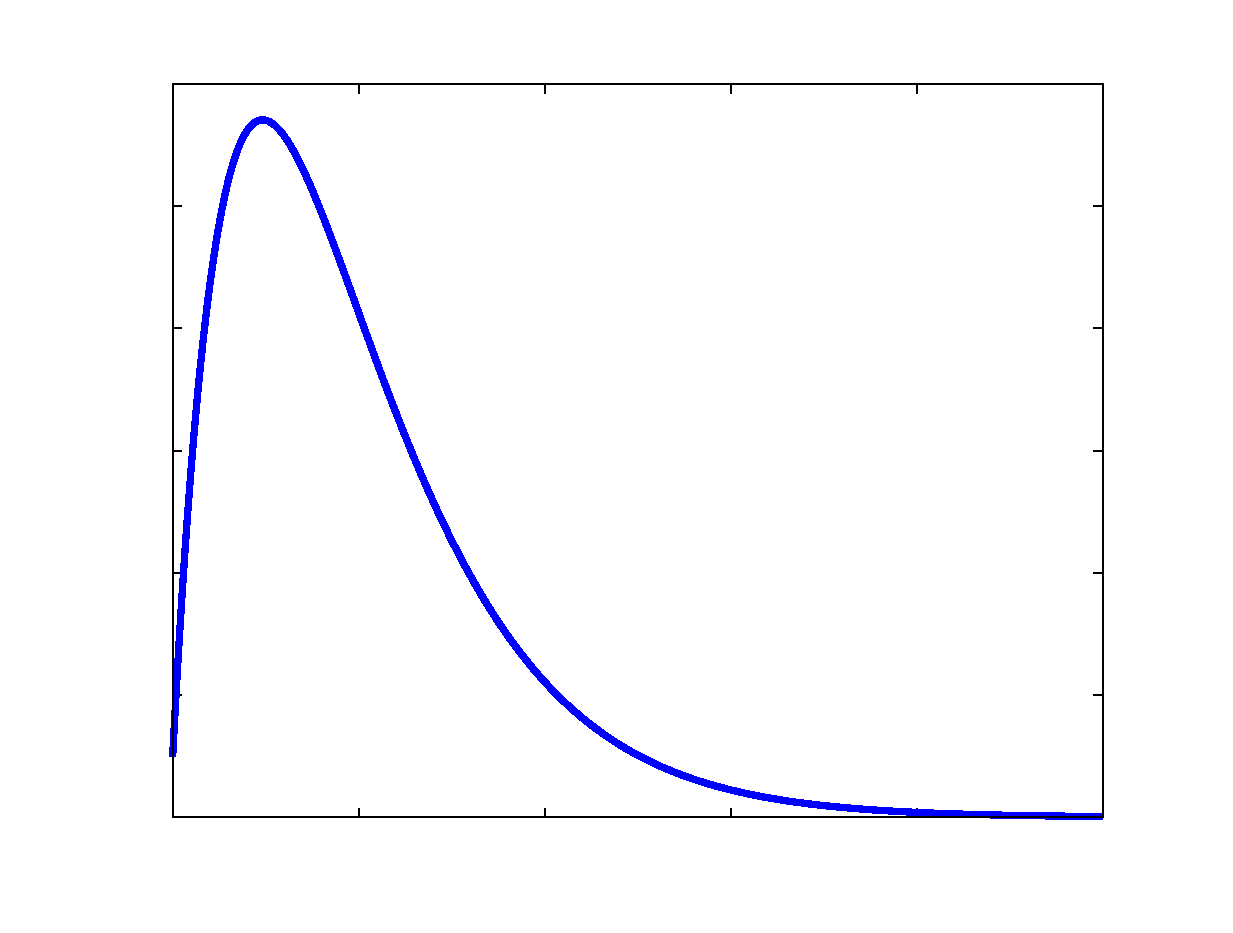
\includegraphics{CriticallyDamped-inc}
\end{picture}%
\begin{picture}(576,432)(0,0)
\fontsize{10}{0}
\selectfont\put(74.8799,42.519){\makebox(0,0)[t]{\textcolor[rgb]{0,0,0}{{0}}}}
\fontsize{10}{0}
\selectfont\put(164.16,42.519){\makebox(0,0)[t]{\textcolor[rgb]{0,0,0}{{20}}}}
\fontsize{10}{0}
\selectfont\put(253.44,42.519){\makebox(0,0)[t]{\textcolor[rgb]{0,0,0}{{40}}}}
\fontsize{10}{0}
\selectfont\put(342.72,42.519){\makebox(0,0)[t]{\textcolor[rgb]{0,0,0}{{60}}}}
\fontsize{10}{0}
\selectfont\put(432,42.519){\makebox(0,0)[t]{\textcolor[rgb]{0,0,0}{{80}}}}
\fontsize{10}{0}
\selectfont\put(521.28,42.519){\makebox(0,0)[t]{\textcolor[rgb]{0,0,0}{{100}}}}
\fontsize{10}{0}
\selectfont\put(69.8755,47.52){\makebox(0,0)[r]{\textcolor[rgb]{0,0,0}{{0}}}}
\fontsize{10}{0}
\selectfont\put(69.8755,106.2){\makebox(0,0)[r]{\textcolor[rgb]{0,0,0}{{2}}}}
\fontsize{10}{0}
\selectfont\put(69.8755,164.88){\makebox(0,0)[r]{\textcolor[rgb]{0,0,0}{{4}}}}
\fontsize{10}{0}
\selectfont\put(69.8755,223.56){\makebox(0,0)[r]{\textcolor[rgb]{0,0,0}{{6}}}}
\fontsize{10}{0}
\selectfont\put(69.8755,282.24){\makebox(0,0)[r]{\textcolor[rgb]{0,0,0}{{8}}}}
\fontsize{10}{0}
\selectfont\put(69.8755,340.92){\makebox(0,0)[r]{\textcolor[rgb]{0,0,0}{{10}}}}
\fontsize{10}{0}
\selectfont\put(69.8755,399.6){\makebox(0,0)[r]{\textcolor[rgb]{0,0,0}{{12}}}}
\end{picture}
}
          \caption{$\Delta=0$}
          \label{fig:0b}
      \end{subfigure} %
      \begin{subfigure}{.3\textwidth}
          \centering
          \scalebox{0.25}{\input{CodigosDibujos/UnderDamped.tex}}
          \caption{$\Delta<0$}
          \label{fig:0c}
      \end{subfigure}
      % 
      \caption{Tipo de soluciones de la ecuación homogénea ($y_h$) dependiendo del signo de $\Delta$.}
      \label{fig:SolucionesHomogenea}
    
\end{figurebox}
\end{figure}

Para terminar de concretar la solución solamente hace falta dar determinados valores a las constantes. Estos valores han de elegirse de modo que se cumplan las condiciones iniciales que impone el circuito. Para esto hay que tener en cuenta las exigencias físicas de los elementos que tenemos, como la inducción y el condensador. En cualquier caso, no nos interesa hacer ese análisis ahora.


\subsection{Solución de la no homogénea} 
Es el momento de resolver la ecuación \eqref{eq:RLC}, de modo que buscamos una función $y_p$ que satisfaga la ecuación \eqref{eq:RLC}, por lo que ha de ser:
\[
L\cdot C \cdot y_p '' (t) + R\cdot C\cdot y_p'(t) + y_p(t) = V_S(t).
\]
Como adelantábamos, no podemos intentar resolver la ecuación si no nos dicen nada más sobre $V_S$, así que tendremos que recurrir a las series de Fourier, siguiendo los tres pasos que hemos establecido anteriormente.

\begin{enumerate}[{\bfseries [1]}]
  \item\textit{\color{blue} Dividir el problema complicado en varios problemas sencillos.}

    En primer lugar, la señal de excitación \textbf{real} siempre va a ser finita, de modo que solo me interesa $V_S(t)$ en un determinado intervalo de tiempo. Ahora bien, la función matemática que utilizamos para representar la señal se puede \textit{extender} a una función periódica (la idea para conseguirlo es ir repitiendo la gráfica hacia los lados).

Con esta aclaración estamos en condiciones de aplicar el teorema de Fourier. Si $V_S$ tiene período $2p$ podemos escribirlo como suma de armónicos:
\[
V_S(t) = a_0 + \sum_{k=0}^{\infty} [a_k \cdot \cos(\omega_kt) + b_k \cdot \sin(\omega_kt)]\qquad \text{donde}\quad \omega_k=\frac{k\cdot \pi}{p}.
\]
  \item \textit{\color{blue}Resolver por separado cada uno de los problemas sencillos.}

Planteamos por separado el caso en el que $V_S$ es una constante, o una suma de cosenos y senos.

 $\clubsuit$ Vamos a hallar $y_0$, solución de:
\[
L\cdot C \,y_0 '' (t) + R\cdot C\, y_0'(t) + y_0(t) = a_0.
\]
En este caso, es fácil ver que
\[\boxed{
y_0(t) = a_0
}\]
cumple los requisitos.

 $\clubsuit$ Ahora vamos a hallar $y_{k}$, solución de:
\[
L\cdot C \,y_k '' (t) + R\cdot C\, y_k'(t) + y_k(t) = a_k\cdot \cos(\omega_kt) +  b_k\cdot \sin(\omega_kt) .
\]
En estos casos, la literatura sugiere probar una solución de la forma:
\[
y_{k}(t) = \alpha_k\cdot \cos(\omega_kt) + \beta_k\cdot \sin(\omega_kt),
\]
donde $\alpha_k$ y $\beta_k$ son coeficientes por determinar. Definimos ahora:
\[
A_k = 1- L\cdot C\omega_k^2,\qquad\text{y}\qquad B_k = R\cdot C\omega_k.
\]
Estos coeficientes son útiles porque si derivamos $y_{k}$ y sustituimos en la ecuación diferencial, obtenemos:
\[
 \left[A_k \cdot \alpha_k + B_k\cdot \beta_k\right] \cos(\omega_k t) + \left[-B_k \cdot \alpha_k + A_k\cdot \beta_k\right] \sin(\omega_k t) = a_k\cdot \cos(\omega_kt) +  b_k\cdot \sin(\omega_kt) ,
\]
de modo que la función propuesta será solución precisamente cuando los coeficientes cumplan el siguiente sistema de ecuaciones que podemos escribir y resolver matricialmente
\[
\left(\begin{array}{cc}
A_k  & B_k\\
-B_k & A_k
\end{array}\right)
\left(\begin{array}{c}
 \alpha_k  \\
 \beta_k
\end{array}\right)
=
\left(\begin{array}{c}
 a_k  \\
 b_k
\end{array}\right)
%
\quad \Longrightarrow \quad
%
\left(\begin{array}{c}
 \alpha_k  \\
 \beta_k
\end{array}\right)
=
\frac{1}{A_k^2+B_k^2}
\left(\begin{array}{c}
 a_k\cdot A_k-b_k\cdot B_k \\
 a_k\cdot B_k + b_k\cdot A_k
\end{array}\right).
\] 
Por lo tanto, la solución queda:
\begin{equation}
  \label{eq:ModoNormal}
  \boxed{
    y_k(t) = \frac{a_k\cdot A_k-b_k\cdot B_k}{A_k^2+B_k^2}\cos(\omega_kt) + \frac{a_k\cdot B_k + b_k\cdot A_k}{A_k^2+B_k^2}\sin(\omega_kt).
  }
\end{equation}

Cada una de estas soluciones recibe el nombre de \textbf{modo normal de orden $\mathbf{k}$}.
 
  \item \textit{\color{blue}Juntar las soluciones para obtener la solución del problema complicado.}

Basta considerar
\[\boxed{
y_p (t)= \sum _{k=0}^{\infty} y_k (t),
}\]
que por construcción, es la solución particular que buscábamos.
\end{enumerate}

\subsection{Interpretación  de las soluciones}
Como hemos mencionado antes, la solución de \eqref{eq:RLC} es suma de dos contribuciones:
\[
v_C(t) = y_h(t) + y_p(t),
\]
que podemos analizar por separado:
\begin{itemize}
  \item $y_h(t)$ se conoce como \textbf{respuesta natural o transitoria} (ahora veremos porqué). Es la contribución inherente al propio circuito y los elementos que lo componen, pues no depende en absoluto de $V_S$.
  \item $y_p(t)$ se conoce como \textbf{respuesta forzada}. Es la respuesta que provocamos en el circuito a causa de la excitación introducida.
\end{itemize}
Desde un punto de vista práctico, podemos pensar que tenemos un \textit{input} $V_S$ al que le queremos aplicar una transformación para obtener $y_p$. Sin embargo, el simple hecho de utilizar el circuito hace que el \textit{output} $v_C$ tenga una contribución extra $y_h$. Ahora bien, resulta que $y_h$ se hace despreciable a medida que pasa el tiempo, más explícitamente:
\[
\lim _{t\rightarrow \infty} y_h (t) = 0,
\]
como se puede comprobar haciendo los correspondientes límites o mirando los ejemplos de la Figura \ref{fig:SolucionesHomogenea}. En consecuencia
\begin{equation}
  \label{eq:aproximacionSolucionRLC}
  v_C(t) \approx y_p(t)\qquad \text{si }t \text{ es suficientemente grande}.
\end{equation}

Como tenemos que esperar hasta alcanzar una solución que se estabilice en el tiempo, decimos que estamos ante un  \textbf{fenómeno transitorio}. La Figura \ref{fig:Transitorio} ilustra esta situación, donde la señal triangular a la salida se ve alterada en los primeros instantes.

\begin{figure}
\begin{figurebox}
    \vspace{0pt}
    \centering
    \scalebox{0.4}{ % Title: glps_renderer figure
% Creator: GL2PS 1.3.8, (C) 1999-2012 C. Geuzaine
% For: Octave
% CreationDate: Mon Jul  7 19:08:28 2014
\setlength{\unitlength}{1pt}
\begin{picture}(0,0)
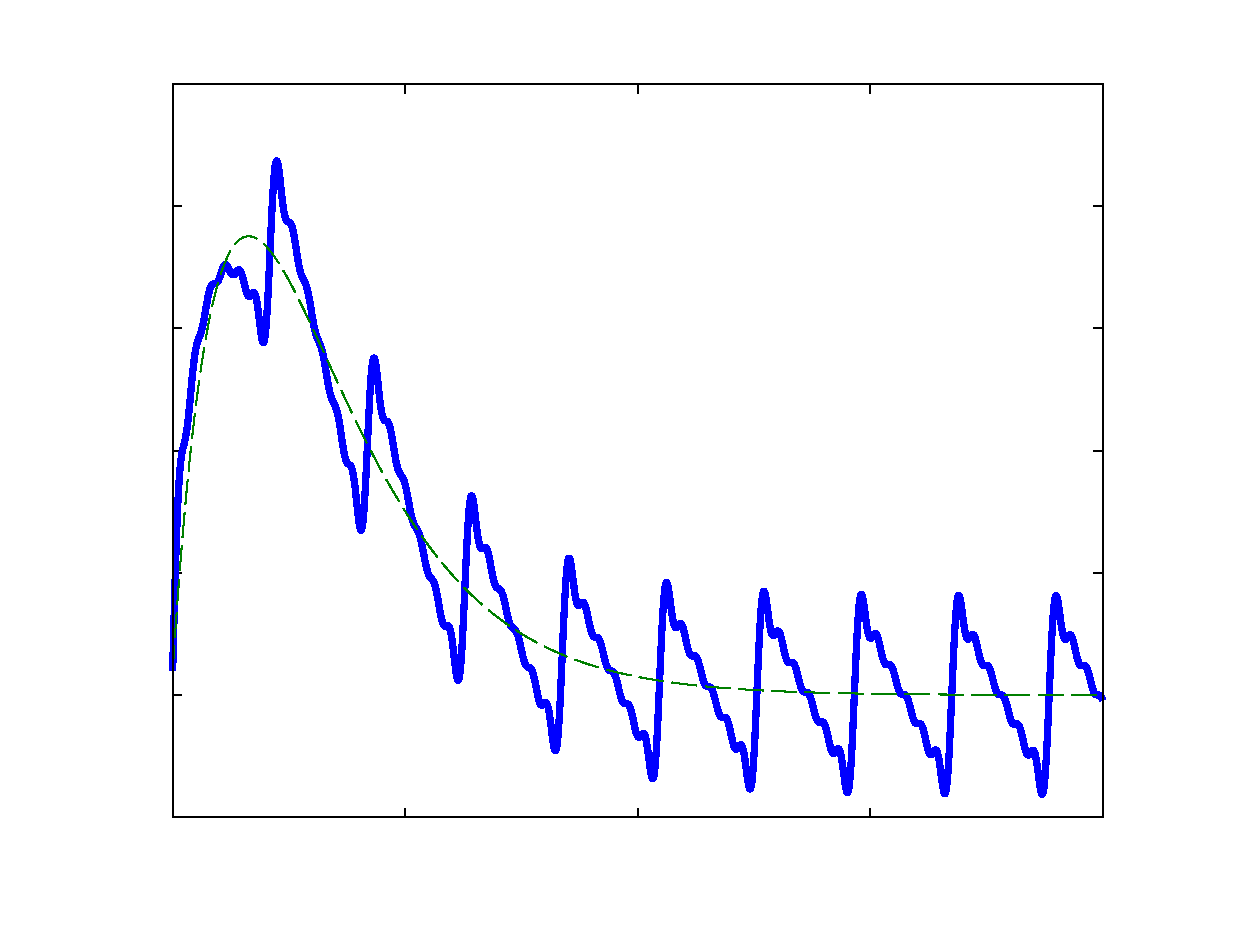
\includegraphics{SumaSoluciones-inc}
\end{picture}%
\begin{picture}(576,432)(0,0)
\fontsize{10}{0}
\selectfont\put(74.8799,42.519){\makebox(0,0)[t]{\textcolor[rgb]{0,0,0}{{0}}}}
\fontsize{10}{0}
\selectfont\put(186.48,42.519){\makebox(0,0)[t]{\textcolor[rgb]{0,0,0}{{50}}}}
\fontsize{10}{0}
\selectfont\put(298.08,42.519){\makebox(0,0)[t]{\textcolor[rgb]{0,0,0}{{100}}}}
\fontsize{10}{0}
\selectfont\put(409.68,42.519){\makebox(0,0)[t]{\textcolor[rgb]{0,0,0}{{150}}}}
\fontsize{10}{0}
\selectfont\put(521.28,42.519){\makebox(0,0)[t]{\textcolor[rgb]{0,0,0}{{200}}}}
\fontsize{10}{0}
\selectfont\put(69.8755,47.52){\makebox(0,0)[r]{\textcolor[rgb]{0,0,0}{{-2}}}}
\fontsize{10}{0}
\selectfont\put(69.8755,106.2){\makebox(0,0)[r]{\textcolor[rgb]{0,0,0}{{0}}}}
\fontsize{10}{0}
\selectfont\put(69.8755,164.88){\makebox(0,0)[r]{\textcolor[rgb]{0,0,0}{{2}}}}
\fontsize{10}{0}
\selectfont\put(69.8755,223.56){\makebox(0,0)[r]{\textcolor[rgb]{0,0,0}{{4}}}}
\fontsize{10}{0}
\selectfont\put(69.8755,282.24){\makebox(0,0)[r]{\textcolor[rgb]{0,0,0}{{6}}}}
\fontsize{10}{0}
\selectfont\put(69.8755,340.92){\makebox(0,0)[r]{\textcolor[rgb]{0,0,0}{{8}}}}
\fontsize{10}{0}
\selectfont\put(69.8755,399.6){\makebox(0,0)[r]{\textcolor[rgb]{0,0,0}{{10}}}}
\end{picture}
}
    \vspace{-10pt}
    \caption{Fenómeno transitorio}
    \label{fig:Transitorio}
\end{figurebox}
\end{figure}





\subsection{Solución final}
Después de todo el trabajo, ya podemos dar una fórmula cerrada para la solución de \eqref{eq:RLC}.
\begin{mybox} \vspace{-4mm}
  \begin{equation}
    \label{eq:SolucionRLC}
    v_C(t) = y_h(t) + \sum _{k=0}^{\infty} y_k (t) = y_h(t) +  \sum _{k=0}^{\infty}  \frac{a_k\cdot A_k-b_k\cdot B_k}{A_k^2+B_k^2}\cos(\omega_kt) + \frac{a_k\cdot B_k + b_k\cdot A_k}{A_k^2+B_k^2}\sin(\omega_kt),
  \end{equation}
  donde $y_h(t)$ es una de las tres opciones descritas en la sección \ref{solucionHomogenea}.
\end{mybox}

Notemos que hemos puesto la misma fórmula para el caso $k=0$, pues en ese caso la excitación es constante, lo que equivale a tomar justo $\omega_0=0$ y se recupera precisamente $y_0=a_0$.

Ya hemos precisado que $y_h(t)$ se hace despreciable a medida que pasa el tiempo, así que también dejaremos escrita la solución \textit{estable en el tiempo}.

\begin{mybox} \vspace{-4mm}
  \begin{equation}
    \label{eq:SolucionRLC2}
    v_C(t) \approx \sum _{k=0}^{\infty}  \frac{a_k\cdot A_k-b_k\cdot B_k}{A_k^2+B_k^2}\cos(\omega_kt) + \frac{a_k\cdot B_k + b_k\cdot A_k}{A_k^2+B_k^2}\sin(\omega_kt).
  \end{equation}
\end{mybox}


\section{Enfoque complejo}

En el anterior artículo descubrimos la relación entre exponenciales complejas y armónicos. Ahora exploraremos cómo llevar a cabo la resolución del circuito sacando provecho de esta idea, llegando al extremo de no tener que resolver ninguna ecuación diferencial. Ahora bien, este método sólo nos permite obtener una solución particular y no tiene en consideración las condiciones iniciales.

Antes de empezar, es necesario hacer una precisión. Cuando se trabaja con circuitos eléctricos, es común representar la unidad imaginaria con la letra $j$ para evitar una posible confusión con la intensidad $i(t)$. De esta manera, escribiremos un número complejo arbitrario como $a+jb\in\mathbb{C}$.

¿Qué sucede si por un momento nos imaginamos que tenemos una señal compleja de la forma $e^{i\omega t}$? Evidentemente, este no será nunca el caso pues las señales son reales, pero ya sabemos que una señal real se puede poner como suma de exponenciales complejas, así que nuestra pregunta tiene sentido. Bajo esta premisa nace la idea de fasor, que analizamos a continuación.

\subsection{Fasores}
Como hemos visto, es muy común trabajar con armónicos a la hora de analizar circuitos eléctricos. Ahora bien, una tensión de la forma $v(t) = V \cos(\omega t + \phi)$ se puede relacionar con exponenciales complejas a través de
\[
v(t) = \frac{V\cdot e^{j(\omega t + \phi)} + V\cdot e^{-j(\omega t + \phi)}}{2}.
\]
Aunque de momento utilizaremos otra relación completamente equivalente que servirá mejor para nuestro propósito:
\[
v(t) = \operatorname{Re} \left[V \cdot e^{j(\omega t + \phi)}\right] = \operatorname{Re} \left [V \cdot e^{j\phi} e^{j\omega t}\right] = \operatorname{Re} \left[\mathbf{V} \cdot  e^{j\omega t}\right],
\]
donde $\mathbf{V} = V \cdot e^{j\phi}$ recibe el nombre de \textbf{fasor}, y es una cantidad compleja que representa a la señal. Como vemos, el fasor sólo nos dice la amplitud y la fase de un armónico. La dependencia temporal se mantiene separada mediante el término $e^{j\omega t}$.

Para la intensidad que circula por el circuito podemos utilizar el mismo criterio\footnote{Si la tensión es un armónico, también lo es la intensidad, consecuencia de las relaciones constitutivas de cada elemento (ver \cite{FasorIntensidad}).} y representarla por medio del fasor $\mathbf{I}$, sabiendo que podemos recuperar el valor real como $i(t)=\operatorname{Re}\left[\mathbf{I}\cdot e^{j\omega t}\right]$.

¿Qué ventajas presenta esto? Veamos cómo expresar las relaciones constitutivas de cada elemento en este contexto.

\begin{itemize}
  \item Cuando hay una resistencia, se tiene una caída de tensión $v_R$ dada por:
    \[
    v_R(t) = i(t)\cdot  R = \operatorname{Re}\left[\mathbf{I}\cdot e^{j\omega t}\right]\cdot R = \operatorname{Re}\left[R\cdot \mathbf{I}\cdot e^{j\omega t}\right],
    \]
    de modo que a la tensión $v_R$ le podemos asociar un fasor relacionado con el de la intensidad por medio de
    \begin{equation}
      \label{eq:FasorVR}
      \mathbf{V}_R = R\cdot \mathbf{I}.
    \end{equation}

  \item Cuando hay una inducción en el circuito, la caída de tensión que presenta $v_L$ viene dada por:
    \[
    v_L(t) = L \cdot \frac{\text{d}i}{\text{d}t}(t) = L \cdot \operatorname{Re} \left[\frac{\text{d} (\mathbf{I}\cdot e^{j\omega t})}{\text{d}t}\right] = L \cdot  \operatorname{Re} \left[j\cdot \omega\cdot \mathbf{I}\cdot e^{j\omega t}\right] =   \operatorname{Re} \left[j\cdot \omega L\cdot \mathbf{I} \cdot e^{j\omega t}\right],
    \]
    de modo que a la tensión $v_L$ le podemos asociar un fasor relacionado con el de la intensidad por medio de
    \begin{equation}
      \label{eq:FasorVL}
      \mathbf{V}_L = j \cdot \omega \cdot L\cdot\mathbf{I}.
    \end{equation}

  \item Cuando hay un condensador en el circuito, la caída de tensión que presenta $v_C$ viene dada por:
    \[
    v_C(t) = \frac{q(t)}{C} \quad \Longrightarrow \quad  \frac{\text{d}v}{\text{d}t}(t) = \frac{i(t)}{C}  \quad \Longrightarrow \quad \operatorname{Re}\left[j\cdot \omega\cdot \mathbf{V}_C\cdot e^{j\omega t}\right] = \operatorname{Re} \left[\frac{\mathbf{I}\cdot e^{j\omega t}}{C}\right],
    \]
    de modo que a la tensión $v_C$ le podemos asociar un fasor relacionado con el de la intensidad por medio de
    \begin{equation}
      \label{eq:FasorVC}
      \mathbf{V}_C = \frac{1}{j\cdot  \omega \cdot C}\,\mathbf{I}.
    \end{equation}
\end{itemize}

\subsection{Impedancia}
Ahora que tenemos los fasores como nueva herramienta, podemos utilizarla para expresar de nuevo la ley de Kirchoff:
\begin{equation}
  \label{eq:KirchoffFasores}
  \mathbf{V}_R + \mathbf{V}_L + \mathbf{V}_C = \mathbf{V}_S,
\end{equation}
y sustituyendo las relaciones \labelcref{eq:FasorVR,eq:FasorVL,eq:FasorVC} en \eqref{eq:KirchoffFasores} encontramos
\[
  \left(R + j\cdot \omega \cdot L + \frac{1}{j\cdot \omega \cdot C}\right) \mathbf{I} = \mathbf{V}_S.
\]
Lo que nos sugiere definir el número complejo
\begin{equation}
  \label{eq:Impedancia}
  \mathbf{Z}=\frac{\mathbf{V}_S}{\mathbf{I}} = R + j\cdot \omega \cdot L + \frac{1}{j\cdot \omega \cdot C},
\end{equation}
conocido como \textbf{impedancia}. En general, se define la impedancia $\mathbf{Z}$ de un circuito o un elemento como el número (generalmente complejo) que satisface:
\begin{equation}
  \label{eq:OhmGeneral}
  \mathbf{V} = \mathbf{I}\cdot \mathbf{Z}.
\end{equation}
Así, podemos entender la impedancia como una generalización del concepto de resistencia, pero englobando también a condensadores e inductores. Por lo tanto, podemos ver también \eqref{eq:OhmGeneral} como una extensión de la ley de Ohm. 

Aquí es donde están empezando a aparecer las diferencias esenciales. Al pasarnos al campo complejo estamos enfrentando un problema donde todos los elementos se comportan esencialmente como resistencias, lo que hace que su resolución sea trivial. Además, el potencial de este método radica en su generalidad, ya que esto lo podemos repetir \textbf{para cualquier circuito}.


\subsection{Resolución}
 Recordemos que nuestro objetivo era hallar la tensión entre las placas del condensador, para lo que sustituimos \eqref{eq:Impedancia} en \eqref{eq:FasorVC}, obteniendo:
\begin{equation}
  \label{eq:SolFasor}
  \mathbf{V}_C = \frac{1}{j\cdot \omega \cdot C} \frac{\mathbf{V_S}}{\mathbf{Z}} =\frac{\frac{1}{j\cdot \omega\cdot C}}{R + j\cdot \omega \cdot L + \frac{1}{j\cdot \omega \cdot C}} \mathbf{V}_S = \frac{1}{(1-\omega^2 \cdot L\cdot C) + j(\omega\cdot R\cdot  C)} \mathbf{V}_S.
\end{equation}

De donde deduciríamos $v_C(t) = \operatorname{Re} \left[\mathbf{V}_C \cdot e^{j\omega t}\right]$. Como esto es válido sólo si la tensión de excitación es una exponencial compleja, en caso real necesitamos aplicar de nuevo nuestra estrategia.

\begin{enumerate}[{\bfseries [1]}]
  \item\textit{\color{blue} Dividir el problema complicado en varios problemas sencillos.}

    Para una excitación genérica, hallamos su serie de Fourier compleja:
    \[
    V_S(t) = \sum_{k=-\infty}^\infty c_k \cdot e^{j\omega_k t},
    \]
    y ya tenemos la excitación como suma de exponenciales complejas. Cada una de ellas se puede representar mediante el fasor $c_k$.
  \item \textit{\color{blue}Resolver por separado cada uno de los problemas sencillos.}

    Para cada contribución, tomamos su fasor y con \eqref{eq:SolFasor} obtenemos el fasor de la solución, de donde:
    \[\boxed{
      \tilde{y}_k (t)= \operatorname{Re}\left[\frac{1}{(1-\omega_k^2 \cdot  L\cdot C) + j(\omega_k R\cdot C)}\ c_k\cdot  e^{j\omega_k t}\right].
    }\]
  \item \textit{\color{blue}Juntar las soluciones para obtener la solución del problema complicado.}

    Simplemente basta hacer
    \[
    v_C(t) =  \sum_{k=-\infty}^\infty \tilde{y}_k(t) = \operatorname{Re}\left[\ \sum_{k=-\infty}^\infty \frac{1}{(1-\omega_k^2 \cdot L\cdot C) + j(\omega_k\cdot R\cdot C)}\cdot  c_k\cdot e^{j\omega_k t}  \right].
    \] 
    Por último, los términos con índices $k$ y $-k$ son conjugados\footnote{En efecto, basta recordar que $c_{-k} = \overline{c_k}$, $\omega_{-k}=-\omega_k$ y que $\overline{e^z}=e^{\overline{z}}$}, así que la suma es un número real y basta poner
    \begin{equation} \boxed{
      \label{eq:SolucionFasores}
      v_C(t) = \sum_{k=-\infty}^\infty \frac{1}{(1-\omega_k^2 \cdot L\cdot C) + j(\omega_k\cdot R\cdot C)}\cdot c_k \cdot e^{j\omega_k t}.
    } \end{equation}
\end{enumerate}




\subsection{Solución final}
Lo que nos ha permitido resolver el problema con rapidez ha sido trabajar en el \textbf{dominio fasorial} o \textbf{dominio de la frecuencia}. Una vez hecho esto, es trivial encontrar \eqref{eq:SolFasor}, y a partir de ahí construir la solución \eqref{eq:SolucionFasores}, que gana en simplicidad pues nos hemos desprendido de tener que considerar partes reales. Simplemente basta multiplicar cada exponencial por una impedancia y sumarlas.

Como decíamos, este método sólo nos proporciona una solución particular, para la que podemos dar la siguiente fórmula cerrada:
\begin{mybox} \vspace{-4mm}
  \begin{equation}
    \label{eq:SolucionRLC3}
    v_C(t) = \sum_{k=-\infty}^\infty \frac{1}{(1-\omega_k^2 \cdot L\cdot C) + j(\omega_k \cdot R\cdot C)}\cdot c_k \cdot e^{j\omega_k t}.
  \end{equation}
\end{mybox}

Este puede ser un buen momento para comprobar que las soluciones \eqref{eq:SolucionRLC2} y \eqref{eq:SolucionRLC3}, obtenidas con dos métodos diferentes, son iguales. Para ello, veamos que $ \tilde{y}_k + \tilde{y}_{-k} = y_k$ siendo $y_k$ lo que definimos en \eqref{eq:ModoNormal} como modo normal.

\begin{align*}
   \tilde{y}_k(t) + \tilde{y}_{-k}(t) 
   &= 2 \tilde{y}_k(t) = 2\operatorname{Re}\left[ \frac{1}{A_k + jB_k}\cdot  \left(\frac{a_k-jb_k}{2}\right)\cdot e^{j\omega_k t} \right] = \operatorname{Re}\left[ \frac{A_k-jB_k}{A_k^2 + B_k^2}\cdot \left(a_k-jb_k\right)\cdot e^{j\omega_k t} \right] \\
   &=  \frac{1}{A_k^2 + B_k^2} \cdot \operatorname{Re}\left[ ((A_k\cdot a_k - B_k\cdot b_k) - j(A_k\cdot b_k + B_k\cdot a_k)) \cdot e^{j\omega_k t} \right] \\
   &= \frac{1}{A_k^2 + B_k^2}\cdot \left[ (A_k\cdot a_k - B_k\cdot b_k)\cos(\omega_k t) + (A_k\cdot b_k + B_k\cdot a_k)\sin(\omega_k t) \right]\\
   &= y_k(t),
\end{align*}
de donde se deduce inmediatamente que
\[
\sum_{k=-\infty}^\infty \tilde{y}_k(t) = \sum_{k=0}^\infty y_k (t),
\]
y que por tanto, las soluciones coinciden.















\section{Resonancia}
Para analizar el circuito RLC hemos tenido que recurrir, por dos caminos distintos, a las series de Fourier. En ambos casos, la consecuencia es que la solución se expresa como una suma infinita de pequeñas contribuciones, cada una asociada a una frecuencia $\omega_k$ diferente.

¿Hay alguna frecuencia que contribuya más que las demás? Para responder a esta pregunta tenemos que analizar la \textbf{respuesta frecuencial}. De la ecuación \eqref{eq:SolFasor} se deduce que cada frecuencia ve multiplicada su amplitud por el término
\begin{equation}
  \label{eq:FuncionTransferencia}
  H(\omega) = \frac{1}{(1-\omega^2 \cdot L\cdot C) + j(\omega \cdot R\cdot C)}.
\end{equation}
La función $H(\omega)$ recibe el nombre de \textbf{función de transferencia} y me dice cuánto crece cada exponencial tras pasar por el circuito. De hecho, como $H(\omega)$ es un número complejo, la información relativa al tamaño está contenida en el módulo:
\begin{equation}
  \label{eq:ModuloFuncionTransferencia}
  \left|H(\omega)\right| = \frac{1}{\sqrt{(1-\omega^2\cdot L\cdot C)^2 + (\omega \cdot R\cdot C)^2}}.
\end{equation}

\begin{figure}
\begin{figurebox}
    \vspace{5pt}
    \centering
    \scalebox{0.4}{ % Title: glps_renderer figure
% Creator: GL2PS 1.3.8, (C) 1999-2012 C. Geuzaine
% For: Octave
% CreationDate: Mon Aug 18 14:41:30 2014
\setlength{\unitlength}{1pt}
\begin{picture}(0,0)
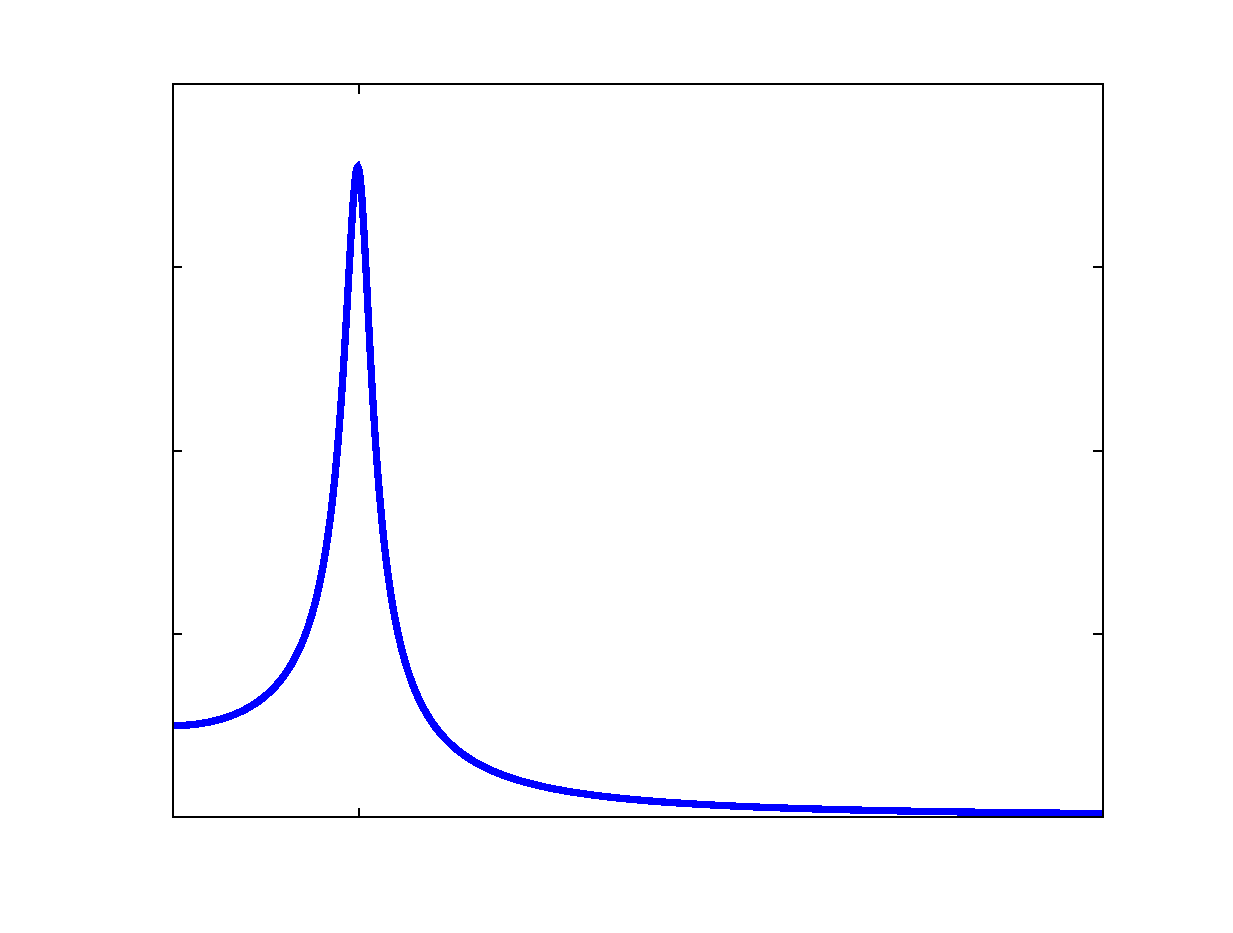
\includegraphics{Resonancia-inc}
\end{picture}%
\begin{picture}(576,432)(0,0)
\fontsize{30}{0}
\selectfont\put(164.16,42.519){\makebox(0,0)[t]{\textcolor[rgb]{0,0,0}{{$\omega_r$}}}}
\fontsize{30}{0}
\selectfont\put(69.8755,47.52){\makebox(0,0)[r]{\textcolor[rgb]{0,0,0}{{0}}}}
\fontsize{30}{0}
\selectfont\put(69.8755,135.54){\makebox(0,0)[r]{\textcolor[rgb]{0,0,0}{{2}}}}
\fontsize{30}{0}
\selectfont\put(69.8755,223.56){\makebox(0,0)[r]{\textcolor[rgb]{0,0,0}{{4}}}}
\fontsize{30}{0}
\selectfont\put(69.8755,311.58){\makebox(0,0)[r]{\textcolor[rgb]{0,0,0}{{6}}}}
\fontsize{30}{0}
\selectfont\put(69.8755,399.6){\makebox(0,0)[r]{\textcolor[rgb]{0,0,0}{{8}}}}
\end{picture}
}
    \vspace{-10pt}
    \caption{Fenómeno de resonancia.}
    \label{fig:Resonancia}
\end{figurebox}
\end{figure}


En la Figura \ref{fig:Resonancia} podemos observar la representación gráfica de \eqref{eq:ModuloFuncionTransferencia}. Como vemos, hay una banda de frecuencias para las cuales $H(\omega)$ es especialmente grande, lo que produce el fenómeno conocido como \textbf{resonancia}. Para caracterizar este fenómeno, se define la \textbf{frecuencia de resonancia} como
\begin{equation}
  \label{eq:FrecuenciaNatural}
  \omega_r = \frac{1}{\sqrt{L\cdot C}}.
\end{equation}
Resulta que cuando $\omega=\omega_r$ la impedancia es un número real y su módulo alcanza su valor mínimo (como se puede comprobar en \eqref{eq:Impedancia}), de modo que la intensidad que circula por el circuito es máxima (consecuencia inmediata de \eqref{eq:OhmGeneral}). Además, en la práctica el coeficiente $R\cdot C$ es muy pequeño, de modo que \eqref{eq:ModuloFuncionTransferencia} alcanza su valor máximo para una frecuencia muy cercana a $\omega_r$.

Por esta y otras razones, la frecuencia de resonancia es un parámetro esencial a la hora de caracterizar un circuito. En lo que sigue vamos a ver una de sus aplicaciones más inmediatas.


\subsection{Filtros pasabanda}
Cuando se trabaja en telecomunicaciones, es común encontrarnos con señales que presentan un nivel de \textbf{ruido} que nos impide recibir la señal con claridad. Ante esta situación sería ideal tener alguna manera de eliminar el ruido, haciendo pasar la señal por un \textbf{filtro}.

Para ilustrar esta situación debemos fijarnos en la Figura \ref{fig:EfectoFiltro}, donde representamos la señal con la que empezamos y la señal a la que queremos llegar.


\begin{figure}[h]
\begin{figurebox}
    \vspace{10pt}
    \centering
      \begin{subfigure}{.45\textwidth}
          \centering
          \scalebox{0.30}{ \input{CodigosDibujos/SignalRuido.tex}}
          \caption{Señal sin filtrar}
          \label{fig:0a} 
      \end{subfigure}%
      \begin{subfigure}{.45\textwidth}
          \centering
          \scalebox{0.30}{% Title: glps_renderer figure
% Creator: GL2PS 1.3.8, (C) 1999-2012 C. Geuzaine
% For: Octave
% CreationDate: Wed Jul  9 15:56:49 2014
\setlength{\unitlength}{1pt}
\begin{picture}(0,0)
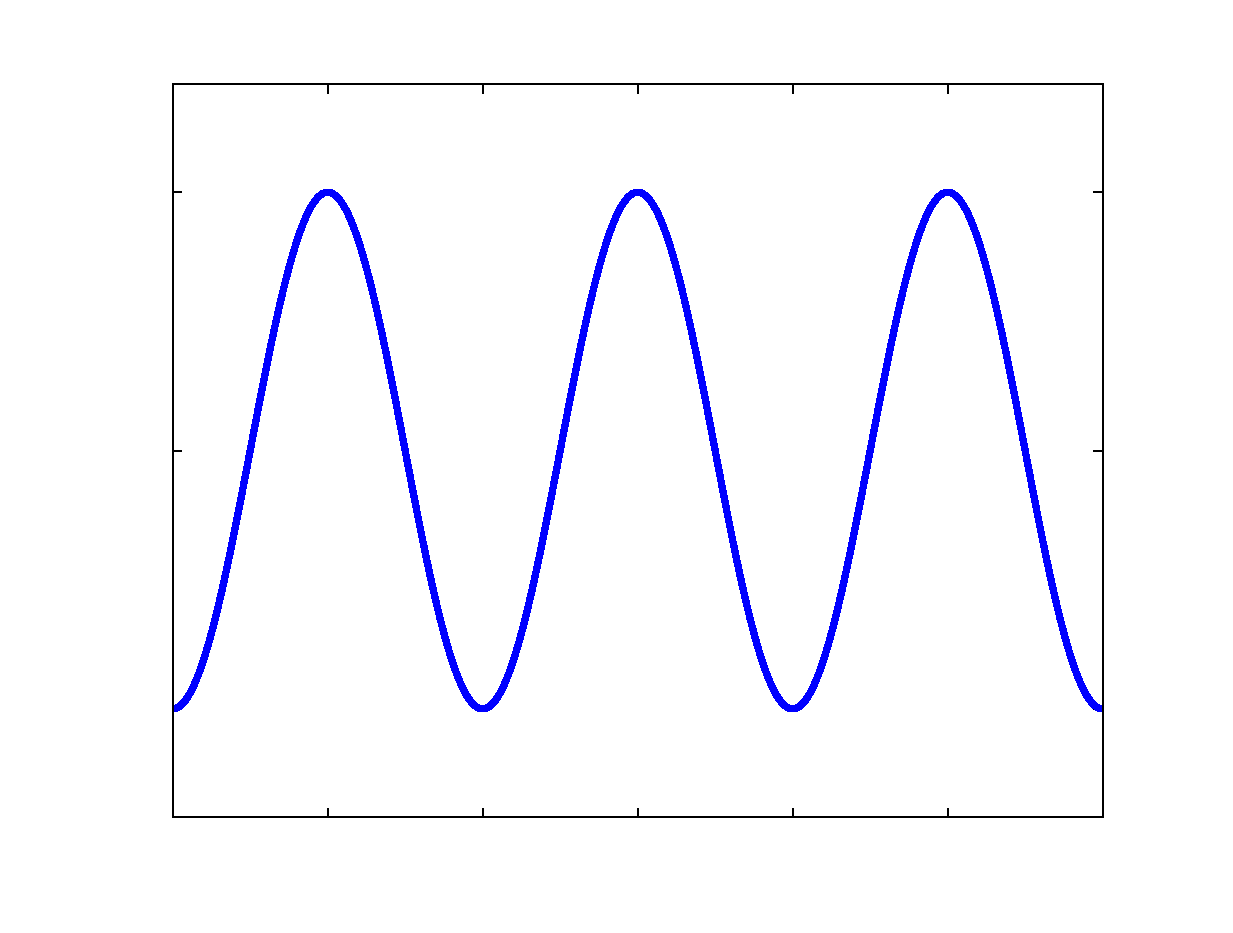
\includegraphics{SignalSinRuido-inc}
\end{picture}%
\begin{picture}(576,432)(0,0)
\fontsize{30}{0}
\selectfont\put(149.28,42.519){\makebox(0,0)[t]{\textcolor[rgb]{0,0,0}{{-2$\pi$}}}}
\fontsize{30}{0}
\selectfont\put(223.68,42.519){\makebox(0,0)[t]{\textcolor[rgb]{0,0,0}{{-$\pi$}}}}
\fontsize{30}{0}
\selectfont\put(298.08,42.519){\makebox(0,0)[t]{\textcolor[rgb]{0,0,0}{{0}}}}
\fontsize{30}{0}
\selectfont\put(372.48,42.519){\makebox(0,0)[t]{\textcolor[rgb]{0,0,0}{{$\pi$}}}}
\fontsize{30}{0}
\selectfont\put(446.88,42.519){\makebox(0,0)[t]{\textcolor[rgb]{0,0,0}{{2$\pi$}}}}
\fontsize{30}{0}
\selectfont\put(69.8755,99.5884){\makebox(0,0)[r]{\textcolor[rgb]{0,0,0}{{-10}}}}
\fontsize{30}{0}
\selectfont\put(69.8755,223.56){\makebox(0,0)[r]{\textcolor[rgb]{0,0,0}{{0}}}}
\fontsize{30}{0}
\selectfont\put(69.8755,347.532){\makebox(0,0)[r]{\textcolor[rgb]{0,0,0}{{10}}}}
\end{picture}
}
          \caption{Señal filtrada}
          \label{fig:0b}
      \end{subfigure}
      \caption{Efecto del filtro sobre una señal con ruido}
      \label{fig:EfectoFiltro}
    
\end{figurebox}
\end{figure}

Ahora vamos a hacer una suposición esencial: \textit{las frecuencias que aparecen al hacer el desarrollo de Fourier del ruido no coinciden con las frecuencias de la señal}. En la práctica, no siempre será legítimo suponer esto\footnote{ En cuyo caso, habría que atacar el problema con un enfoque distinto.}, ya que depende de la naturaleza de la señal y del tipo de ruido (más sobre tipos de ruido en \cite{ColorNoise}). De esta manera, tendremos una función a la cual podemos hacerle el desarrollo en serie de Fourier, que escribimos distinguiendo explícitamente las frecuencias que componen el ruido.
\begin{equation}
  \label{eq:FourierSignalRuido1}
  f(t) = \sum_{\omega_k\text{ de la señal}}\!\!\!\!\!\!\!c_k \cdot e^{j\omega_k t}\ \ +\  \sum_{\omega_k\text{ del ruido}}\!\!\!\!\!c_k \cdot e^{j\omega_k t}.
\end{equation}

Por simplicidad, podemos suponer además que el primer sumatorio de \eqref{eq:FourierSignalRuido} está compuesto por un sólo término de frecuencia $\omega_r$, de modo que el desarrollo de Fourier queda
\begin{equation}
  \label{eq:FourierSignalRuido}
  f(t) = c_r \cdot e^{j\omega_r t}\ \ +\  \sum_{\omega_k\text{ del ruido}}\!\!\!\!\!c_k \cdot e^{j\omega_k t}.
\end{equation}

Ahora basta que hagamos pasar la señal por un circuito RLC. De esta manera, la señal a la salida viene dada por \eqref{eq:SolucionRLC3}, y en este caso queda:
\begin{equation}
  \label{eq:FourierSignalFiltrada1}
  v_C(t) = H(\omega_r) \cdot c_r \cdot e^{j\omega_r t}\ \ +\  \sum_{\omega_k\text{ del ruido}}\!\!\!\!\! H(\omega_k)\cdot c_k\cdot e^{j\omega_k t}.
\end{equation}
 Ahora bien, si elegimos los valores de $L$ y de $C$ de modo que la frecuencia $\omega_r$ sea precisamente la frecuencia de resonancia del circuito (es decir, $\omega_r = \frac{1}{\sqrt{L\cdot C}}$), tendremos que:
 \begin{itemize}
 \item $H(\omega_r)$ será relativamente alto (por ejemplo, en la Figura \ref{fig:Resonancia}, sería $H(\omega_r)\approx 7$).
 \item $H(\omega_k)$ será casi nulo, ya que las frecuencias del ruido están lejos de $\omega_r$. Así  $H(\omega_k)\approx 0$.
 \end{itemize}
En consecuencia tenemos que la señal tras pasar por el circuito es aproximadamente:
\begin{mybox}\vspace{-15pt}
  \begin{equation}
    \label{eq:FourierSignalFiltrada}
    v_C(t) \approx H(\omega_r) \cdot c_r \cdot e^{j\omega_r t}.
  \end{equation}
\end{mybox}

Por esta razón decimos que el circuito funciona como \textbf{filtro}. En particular, se dice filtro pasabanda porque solo mantiene las frecuencias que están en una banda centrada en $\omega_r$ (fuera de la banda, $H(\omega)\approx 0$). Si nuestra señal es un poco más complicada, seguramente exista un filtro más complicado que se adapte a nuestras necesidades. Algunos ejemplos típicos son los filtros pasa-baja, que mantienen todos las frecuencias por debajo de una frecuencia umbral, filtros pasa-alta, filtros rechaza-banda, así como combinaciones de los anteriores.


\bibliographystyle{plain}
\bibliography{fourier1}

\newpage

%%% Local Variables: 
%%% mode: latex
%%% TeX-master: "matematicaseningenieria"
%%% End: 


